\documentclass{beamer}

\usepackage[utf8]{inputenc}
\usepackage[T1]{fontenc}
\usepackage[english]{babel}
\usepackage{lmodern}
\usepackage{algorithm}
\usepackage{algorithmic}

\usetheme{UOS}

\graphicspath{{images/}}

\renewcommand{\baselinestretch}{1.25}

\begin{document}

\title{Normal Calculation in Point Clouds with CUDA}
\author[Alexander Mock, Matthias Greshake]{Alexander Mock, Matthias Greshake\\ {\scriptsize amock@uos.de, mgreshake@uos.de}}
\institute{Institut für Informatik\\ AG Wissensbasierte Systeme}
\date{26. January 2016}

\begin{frame}[plain]
	\titlepage
\end{frame}

\begin{frame}{Outline}
	\tableofcontents
\end{frame}

\begin{frame}{Motivation}
\end{frame}

\begin{frame}{Point Clouds}
	\begin{columns}
		\begin{column}{0.5\textwidth}
			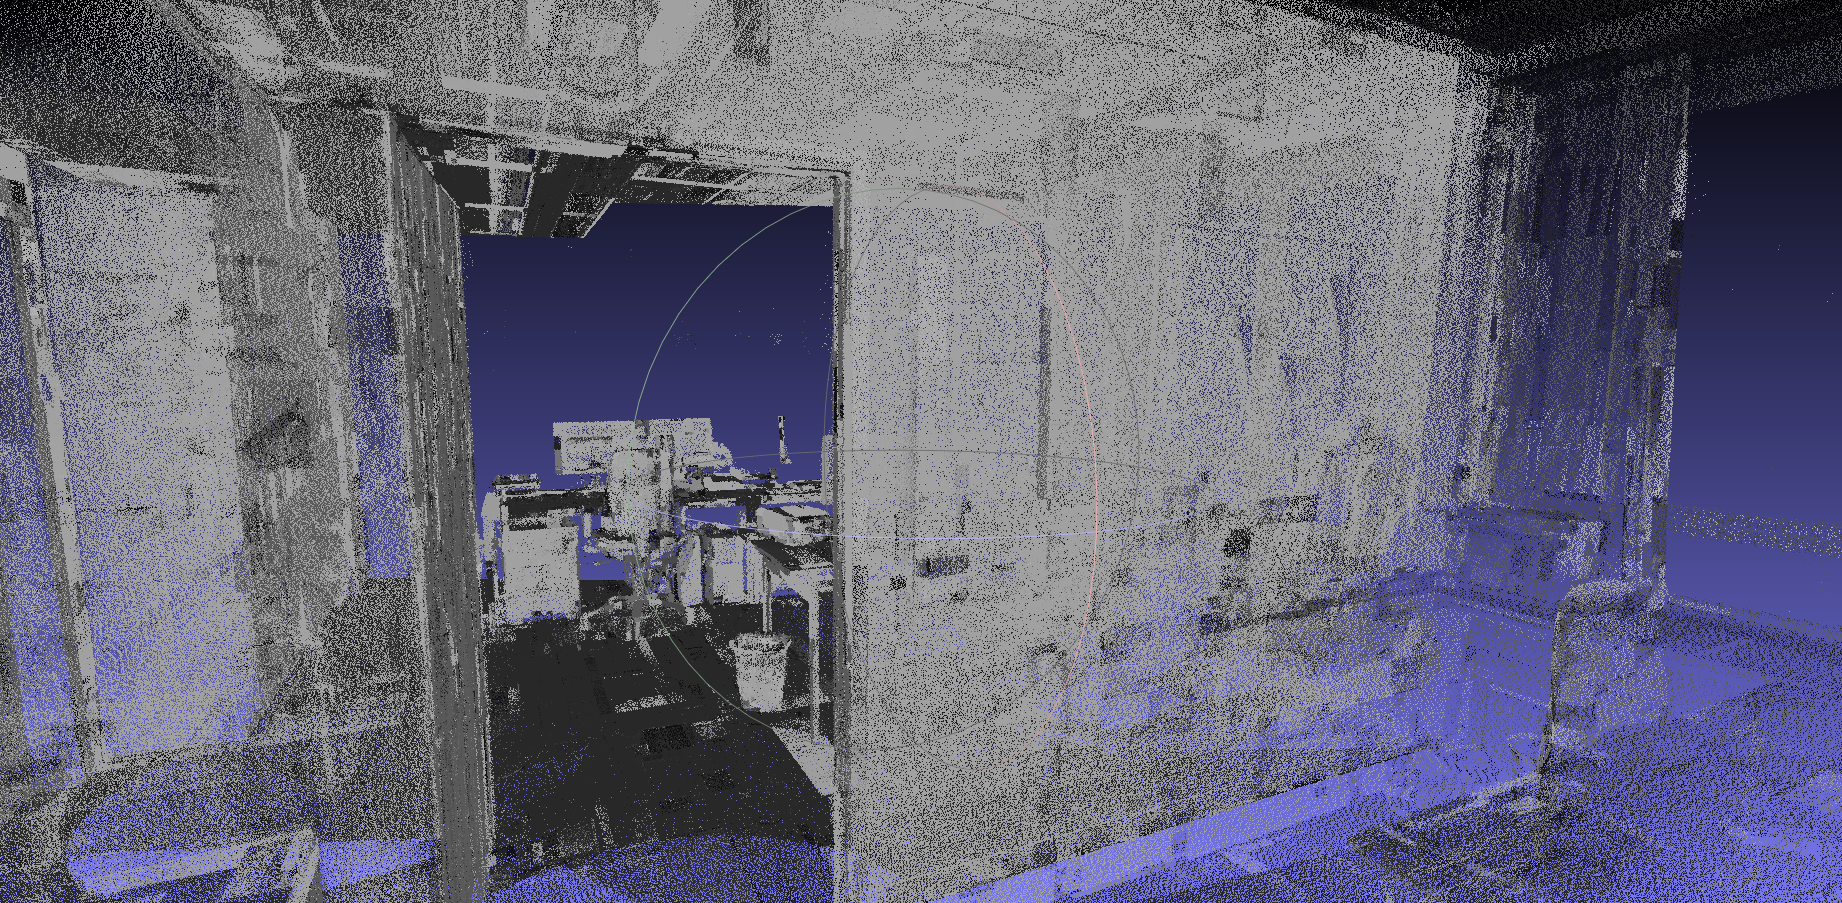
\includegraphics[width=1.0\textwidth]{police_point_cloud.png}
		\end{column}
		\begin{column}{0.5\textwidth}
			\begin{itemize}
				\item Generated by depth sensors of 3D laser scanners
				\item 3D points with geometry data of the environment
				\item No topological connection between points
				\item Polygon meshes based on point clouds
			\end{itemize}
		\end{column}
	\end{columns}
\end{frame}

\begin{frame}{Reconstruction}
	\begin{columns}
		\begin{column}{0.5\textwidth}
			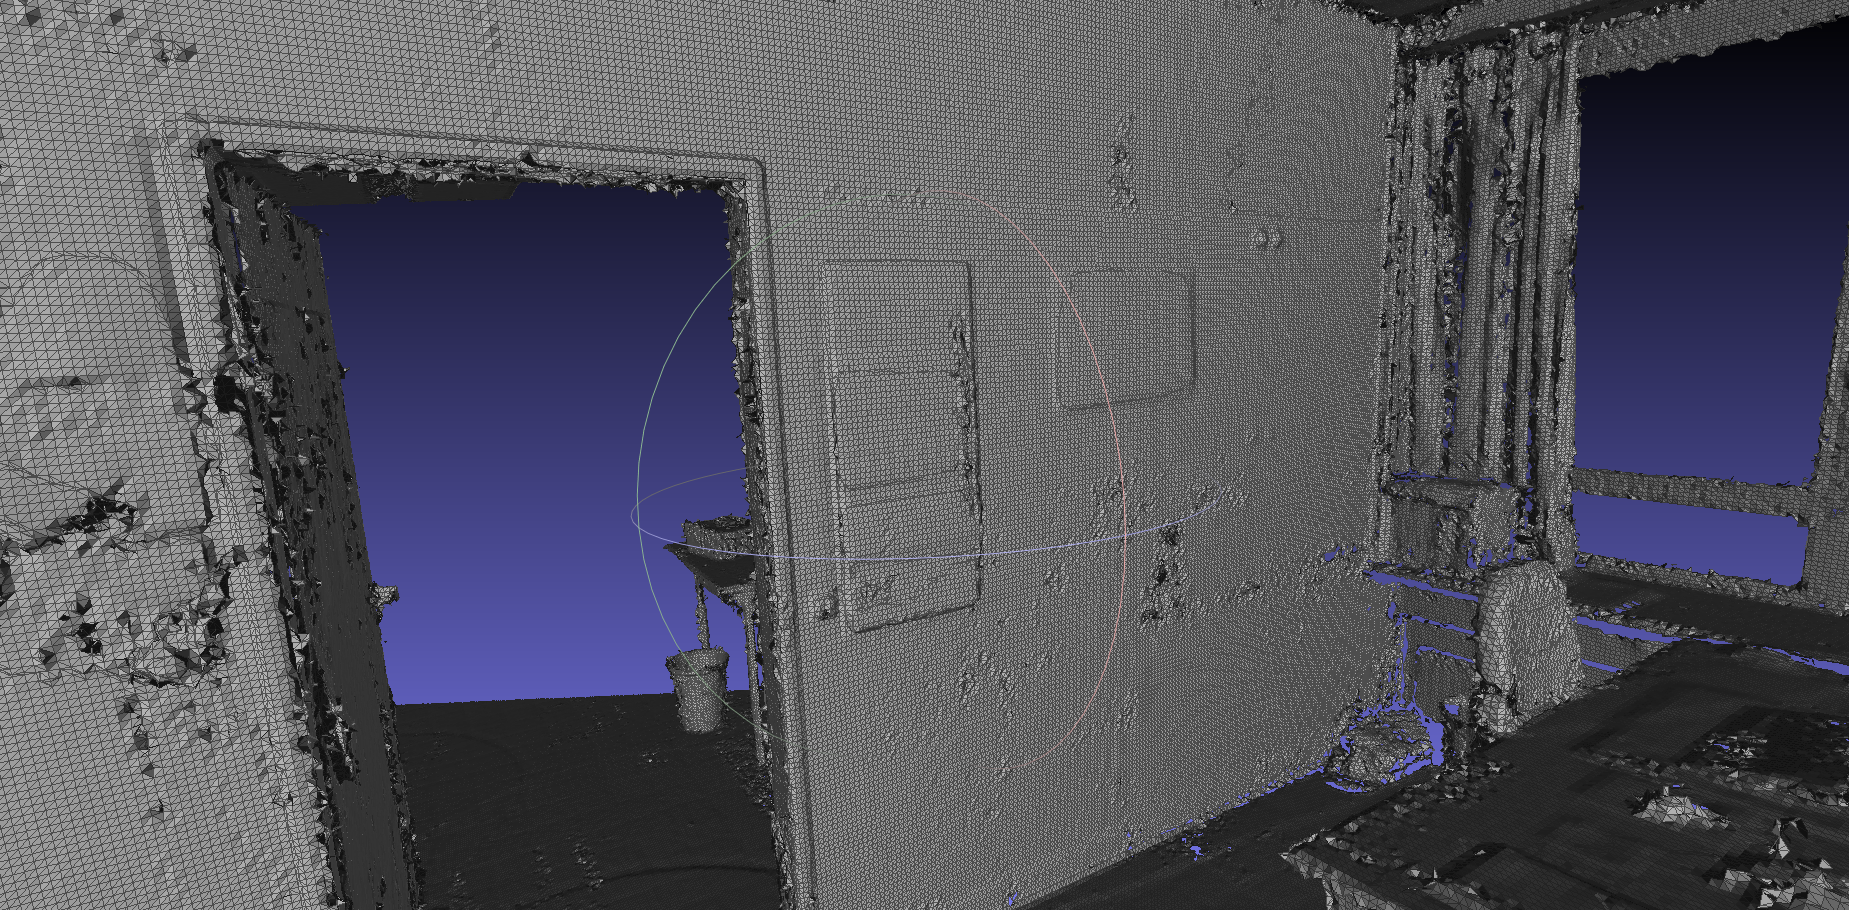
\includegraphics[width=1.0\textwidth]{police_mesh.png}
		\end{column}
		\begin{column}{0.5\textwidth}
			\begin{itemize}
				\item Lower memory usage without loss of information
				\item Normal of each point is necessary to create mesh
				\item Pre-calculation of normals is possible
				\item Requires nearest neighbours of each point
			\end{itemize}
		\end{column}
	\end{columns}
\end{frame}

\section{Problem Statement}

\begin{frame}{Nearest Neighbor Search}
	\begin{itemize}
		\item Independent search of k nearest neighbors to each point
		\item Long runtimes on large datasets
		\begin{block}{}
			\centering Nearest neighbor search is the bottleneck of normal calculation
		\end{block}
		\item Thread-based CPU implementation in the LVR Framework
	\end{itemize}
	\medskip
	\centering $\Rightarrow$ Parallel implementation on GPU to reduce runtime
\end{frame}

\begin{frame}{GPU vs. CPU}
	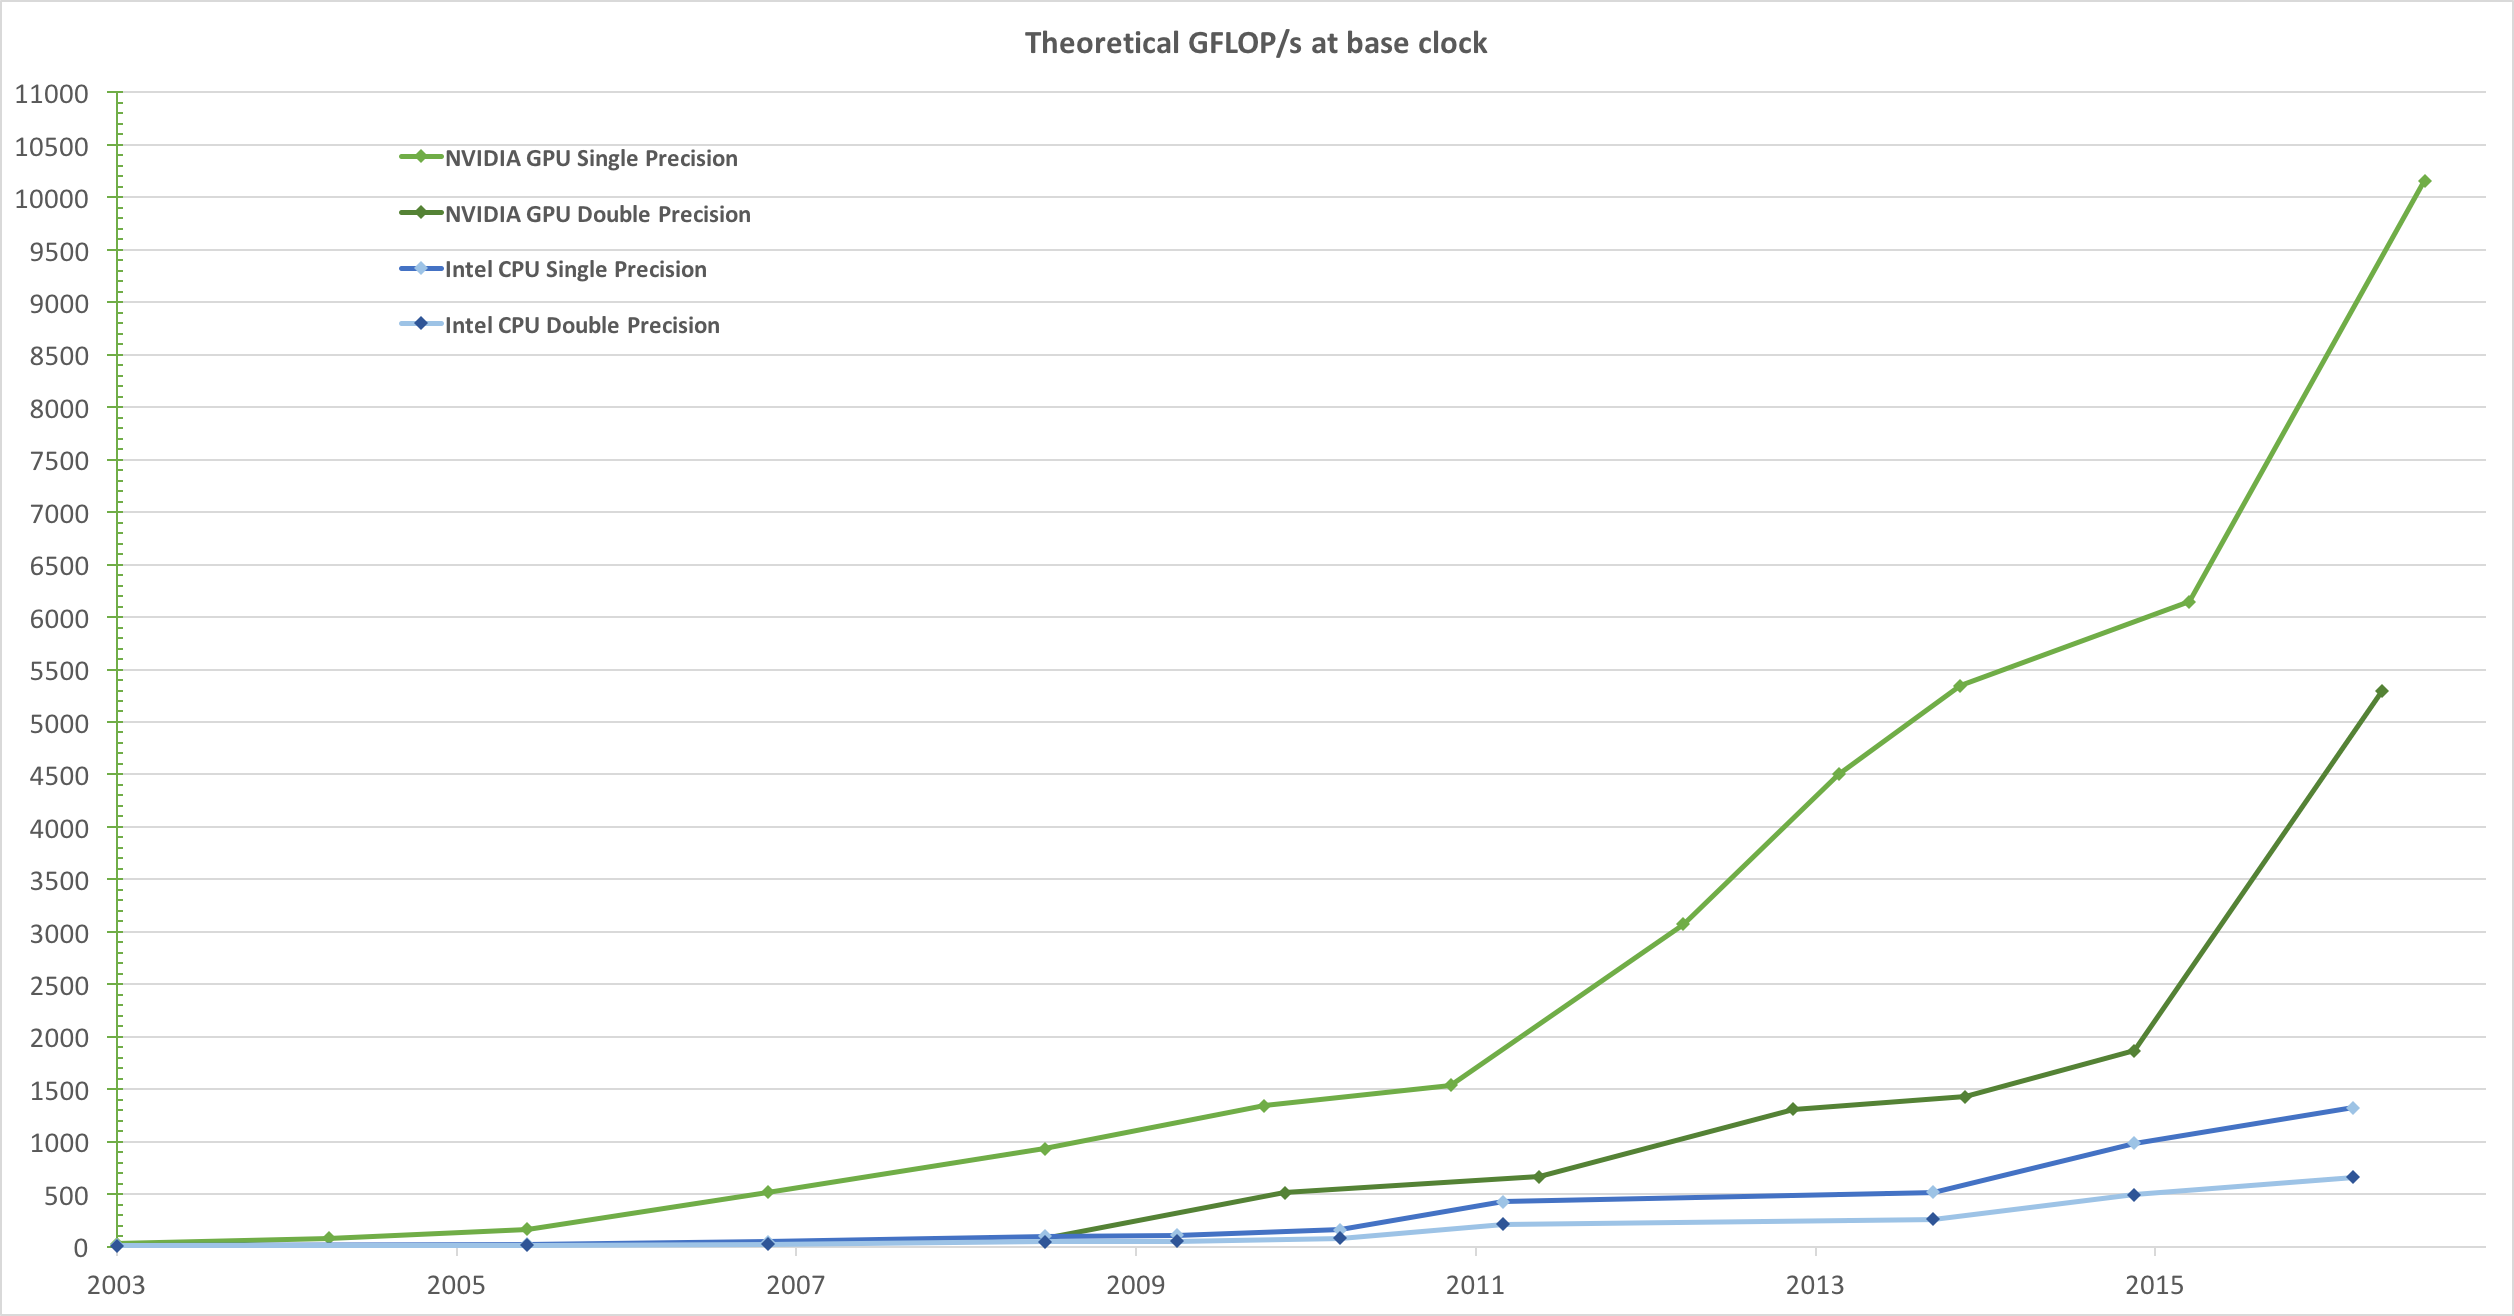
\includegraphics[width=1.0\textwidth]{gpu_comparison.png}
\end{frame}

\subsection*{CUDA}

\begin{frame}{CUDA}
	\begin{columns}[T]
		\begin{column}{0.8\textwidth}
			\begin{itemize}
				\item API for parallel computing on the GPU
				\item Developed by NVIDIA in 2007 
				\item Newest version: 8.0
				\item Supports programming languages C/C++, Fortran, Python and many more
			\end{itemize}
		\end{column}
		\begin{column}{0.2\textwidth}
			
\includegraphics[width=1.0\textwidth]{cuda_logo.jpg}
		\end{column}
	\end{columns}
\end{frame}

\begin{frame}{Threads}
	\begin{columns}
		\begin{column}{0.45\textwidth}
			\centering 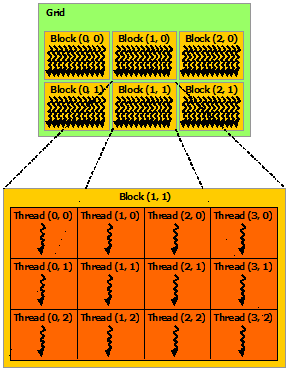
\includegraphics[width=0.9\textwidth]{cuda_threads.png}
		\end{column}
		\begin{column}{0.55\textwidth}
			\begin{itemize}
				\item Parallelization via "Device Kernels" with threads
				\item Organized in blocks on a grid
				\item Block contains 1024 threads at maximum
				\item Blocks have access to shared memory
			\end{itemize}
		\end{column}
	\end{columns}
\end{frame}

\begin{frame}{Memory}
	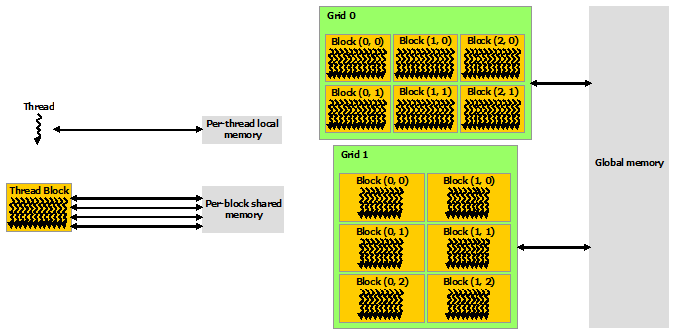
\includegraphics[width=1.0\textwidth]{cuda_memory.png}
\end{frame}

\begin{frame}{Example}
\end{frame}

\subsection*{k Nearest Neighbors}

\begin{frame}{Parallel kNN Search}
	\begin{columns}[T]
		\begin{column}{0.5\textwidth}
			\textbf{Naive Search}
			\begin{itemize}
				\item Highly parallelisable
				\item Low memory usage
				\item Quadratic runtime
				\item 
			\end{itemize}
		\end{column}
		\begin{column}{0.5\textwidth}
			\textbf{kd-Tree}
			\begin{itemize}
				\item Only partial parallelisable
				\item Additional memory for tree representation necessary
				\item Linear runtime for small k
				\item 
			\end{itemize}
		\end{column}
	\end{columns}
\end{frame}

\subsection*{Naive Search}

\begin{frame}{Basic Idea}
	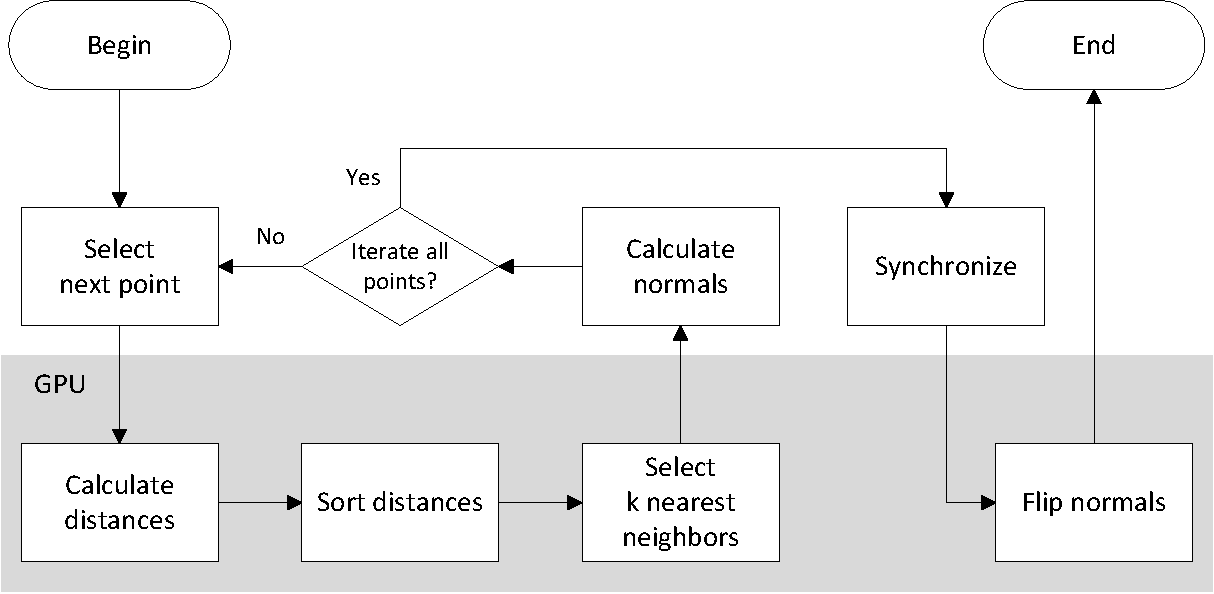
\includegraphics[width=1.0\textwidth]{knn_procedure.pdf}
\end{frame}

\begin{frame}{Implementation}
	\begin{algorithmic}
		\FORALL{points in data}
			\only<1>{\STATE calculate distances to all other points}
			\only<2>{\STATE \textcolor{red}{calculate distances to all other points}}
			\REPEAT
				\STATE count neighbors in radius of $\varepsilon$
				\STATE adapt $\varepsilon = \varepsilon \cdot (1 \pm \eta)$
			\UNTIL{number of neighbors in radius $\varepsilon = k$}
			\STATE get points in radius of $\varepsilon$
		\ENDFOR
	\end{algorithmic}
\end{frame}

\begin{frame}{Distance Calculation}
	\begin{columns}
		\begin{column}{0.5\textwidth}
			\begin{center}
				\only<1>{
				$\begin{pmatrix}
					6 & 0 & 1 & 6\\
					2 & 5 & 7 & 9\\
					4 & 5 & 9 & 4
				\end{pmatrix}$}
				\only<2->{
				$\begin{pmatrix}
					\textcolor{red}{6} & 0 & 1 & 6\\
					\textcolor{red}{2} & 5 & 7 & 9\\
					\textcolor{red}{4} & 5 & 9 & 4
				\end{pmatrix}$\\}
				\uncover<3->{$\Downarrow$\\
				$\begin{pmatrix}
					0 & 6 & 5 & 0\\
					0 & 3 & 5 & 7\\
					0 & 1 & 5 & 0
				\end{pmatrix}$\\}
				\uncover<4>{$\Downarrow$\\
				$\begin{pmatrix}
					0 & 46 & 75 & 49
				\end{pmatrix}$}
			\end{center}
		\end{column}
		\begin{column}{0.5\textwidth}
			\begin{enumerate}
				\item \uncover<2->{Select point from matrix}
				\item \uncover<3->{Determine absolute to each point dimension-wise}
				\item \uncover<4>{Calculate $d = x^2 + y^2 + z^2$}
			\end{enumerate}
		\end{column}
	\end{columns}
\end{frame}

\begin{frame}{Implementation}
	\begin{algorithmic}
		\FORALL{points in data}
			\STATE calculate distances to all other points
			\REPEAT
				\only<1>{\STATE count neighbors in radius of $\varepsilon$
				\STATE adapt $\varepsilon = \varepsilon \cdot (1 \pm \eta)$}
				\only<2>{\STATE \textcolor{red}{count neighbors in radius of $\varepsilon$}
				\STATE \textcolor{red}{adapt $\varepsilon = \varepsilon \cdot (1 \pm \eta)$}}
			\UNTIL{number of neighbors in radius $\varepsilon = k$}
			\STATE get points in radius of $\varepsilon$
		\ENDFOR
	\end{algorithmic}
\end{frame}

\begin{frame}{Distance "Sorting"}
	\begin{columns}
		\begin{column}{0.5\textwidth}
			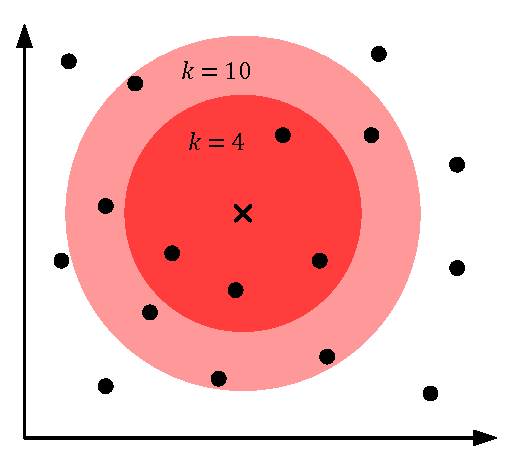
\includegraphics[width=1.0\textwidth]{radius_search.pdf}
		\end{column}
		\begin{column}{0.5\textwidth}
		\begin{itemize}
			\item conventional sorting algorithms not applicable with parallel GPU computing
			\item evaluate a distance $\varepsilon$ based on radius search
			\item count $k$ inside radius $\varepsilon$
			\item adapt $\varepsilon$ iteratively with learning rate $\eta$
		\end{itemize}
		\end{column}
	\end{columns}
\end{frame}

\subsection*{kd-Tree}

\begin{frame}{Kd-tree}
 
\end{frame}

\begin{frame}{GPU-Implementation}
 
\end{frame}

\begin{frame}{Array based left balanced kd-tree}
 
\end{frame}

\begin{frame}{GPU}
 
\end{frame}

\begin{frame}{Kd-tree search}
 
\end{frame}

\begin{frame}{Kd-tree Knn}
 
\end{frame}

\subsection*{Normal Calculation}
\begin{frame}{Normal Calculation}
 
\end{frame}

\begin{frame}{Normal Flip}
 
\end{frame}

\section{Experiment Results}
\subsection*{Results in LVR-Pipeline}
\begin{frame}{Results in LVR-Pipeline}
 \begin{figure}
  \centering
  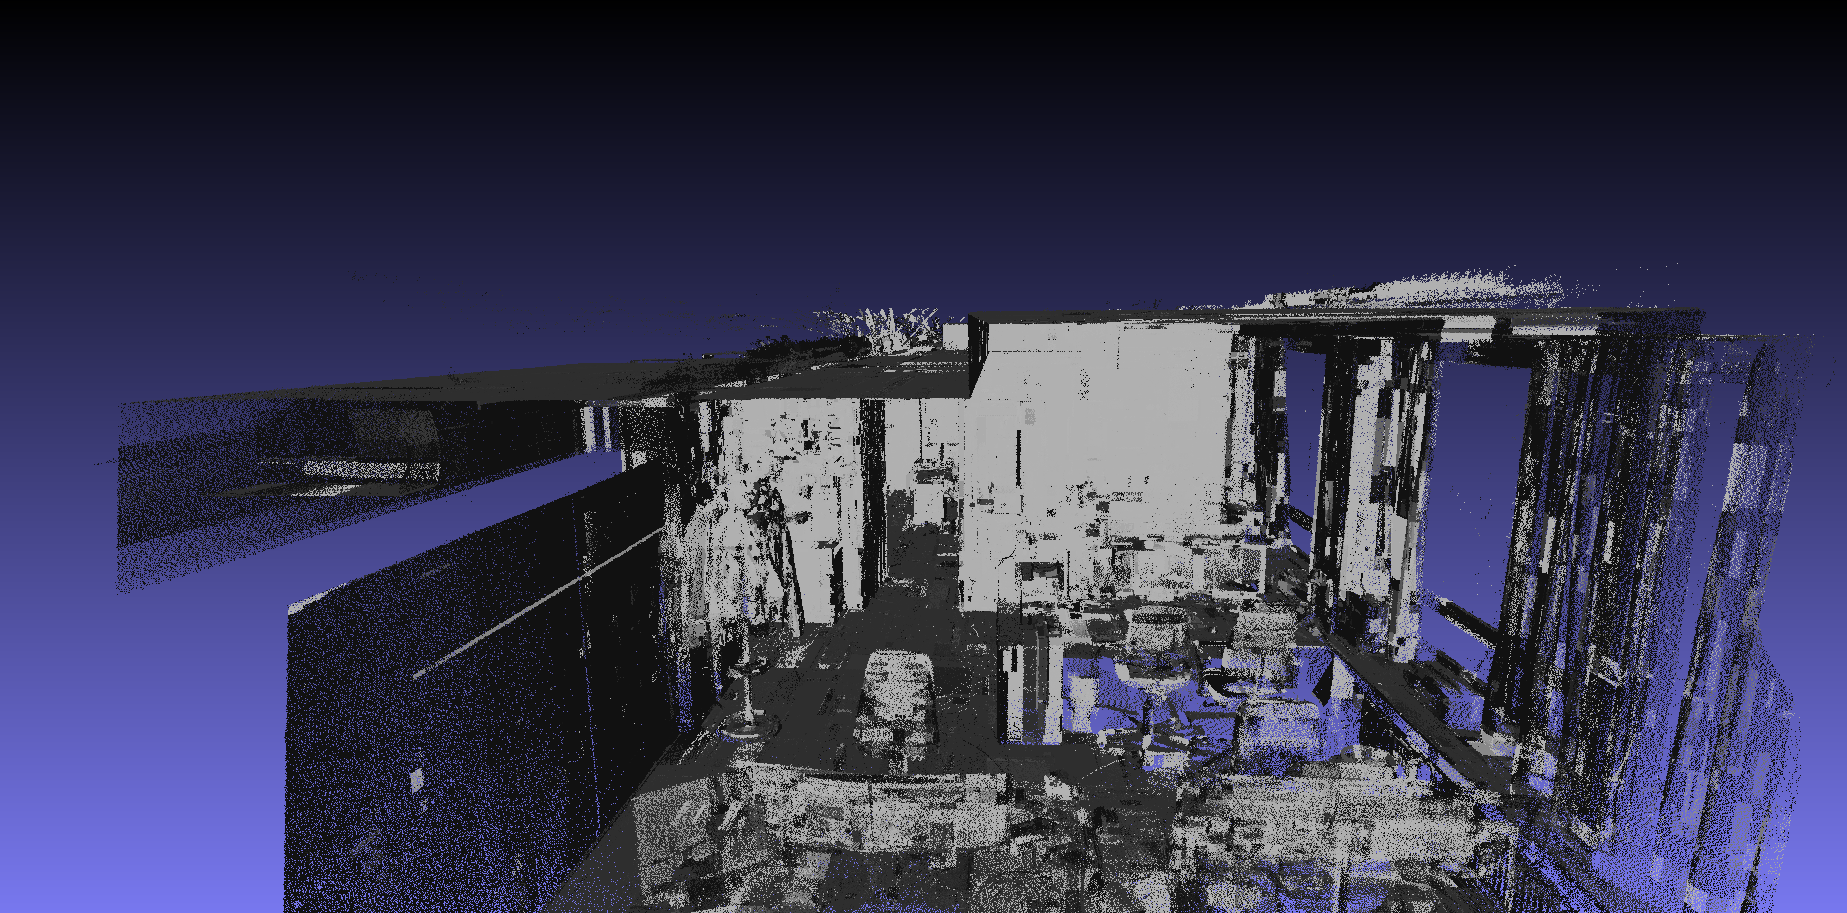
\includegraphics[height=0.4\textheight]{police_no_normals.png}\\
  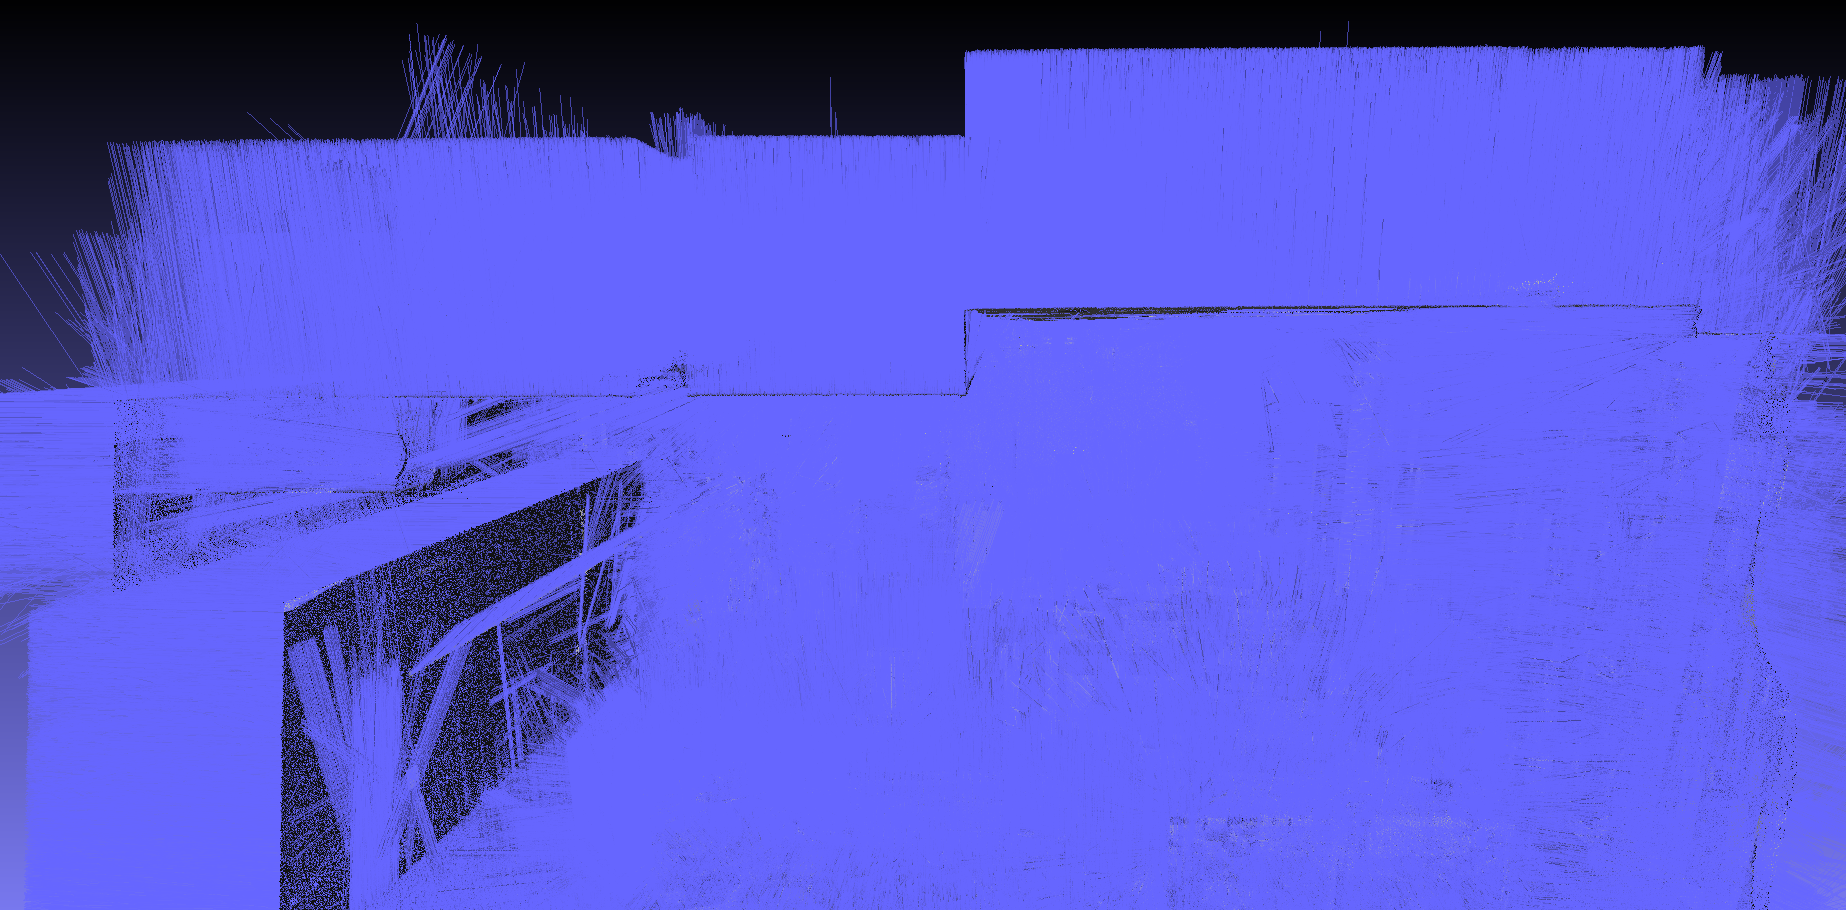
\includegraphics[height=0.4\textheight]{police_normals.png}
 \end{figure}

\end{frame}

\subsection*{Runtime results}
\begin{frame}{Runtime results}
 
\end{frame}

\section{Conclusion}
\begin{frame}{Conclusion}
 
\end{frame}

\end{document}
